\documentclass{article}
\usepackage[a4paper, margin=2cm]{geometry}

\usepackage{amsmath}
\usepackage{amssymb}
\usepackage{mathtools}
\usepackage{amstext}
\usepackage{amsthm}
\usepackage{fancyhdr}
\usepackage{centernot}
\usepackage[ruled,vlined]{algorithm2e}

\usepackage{hyperref}

\usepackage{graphicx}
\usepackage{float}
\usepackage{caption}
\usepackage{subcaption}

\usepackage{booktabs, multirow}

\usepackage{tikz}
\usetikzlibrary{patterns}
\usepackage{pgfplots}
\pgfplotsset{compat=1.15}
\usetikzlibrary{arrows}

% To work with inkfigures
\usepackage{import}
\usepackage{pdfpages}
\usepackage{transparent}
\usepackage{xcolor}

\newcommand{\incfig}[2][1]{%
    \def\svgwidth{#1\columnwidth}
    \import{./figures/}{#2.pdf_tex}
}

\pdfsuppresswarningpagegroup=1

%\graphicspath{{figures/}}

\pagestyle{fancy}
\rhead{Alexandre Adam}
\lhead{Probabilistic Graphical Models \\ Simon Lacoste-Julien}
\chead{Homework 3}
\rfoot{\today}
\cfoot{\thepage}

\newcommand{\angstrom}{\textup{\AA}}
\numberwithin{equation}{section}
\renewcommand\thesubsection{\alph{subsection})}
\renewcommand\thesubsubsection{\Roman{subsubsection}}
\newcommand{\s}{\hspace{0.1cm}}

\newcommand{\indep}{\s \rotatebox[origin=c]{90}{$\models$}\s }

%\tikzset{%
        %observed/.style={pattern=north west lines, pattern color=gray}
        %active_path/.style={->|, dashed, thick, blue}
%}

\tikzset{>=latex}

\begin{document}
\section{DGM}
We consider $G$, a DAG:
\begin{figure}[H]
        \centering
        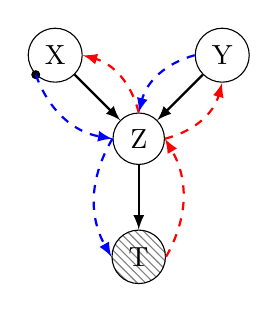
\begin{tikzpicture}
                % cbr = child below right, pbl = parent below left (snippets)
                \tikzstyle{every node}=[circle, draw=black, node distance=1.5cm]
                \tikzstyle{every edge}=[black, ->, thick, draw]
                \node (Z) at (0, 0) {Z};
                \node (Y) [above right of = Z] {Y};
                \draw (Y) edge (Z);
                \node (X) [above left of = Z] {X};
                \draw (X) edge (Z);
                \node[pattern=north west lines, pattern color=gray] (T) [below of = Z] {T};
                \draw (Z) edge (T);
                \node[circle, fill=black, inner sep=1pt] at (X.south west) {}; 

                % bayes ball

                \draw[->, blue, dashed, thick, bend right] (X.south west) to 
                        (Z.west);


                \draw[->, blue, dashed, thick, bend right] (Z.west) to 
                        (T.west);

                \draw[->, red, dashed, thick, bend right] (T.east) to 
                        (Z.east);

                \draw[->, red, dashed, thick, bend right] (Z.east) to 
                        (Y.south);

                
                \draw[->, blue, dashed, thick, bend right] (Y.west) to 
                        (Z.north);

                \draw[->, red, dashed, thick, bend right] (Z.north) to 
                        (X.east);
                
        \end{tikzpicture}
        \caption{Graph $G$, where $T$ is observed. An active path (blue dashed line) can lead 
        from $X$ to $Y$ since this is an undirected path. The arrow is there to indicate the 
        motion of the Bayes Ball. The starting point of the algorithm is represented as a 
black dot.}
        \label{fig:DGM1}
\end{figure}
To prove that $X \indep Y \mid T$, we use the Bayes Ball algorithm (see algorithm 
\ref{alg:Bayes} in the appendix). We conclude that $\boxed{X \centernot\indep Y 
\mid T}$ because there exists an undirected active path (blue dashed line in figure 
\ref{fig:DGM1}) from $X$ to $Y$. This could also have been observed using the fact that
the unobserved node $Z$ with two parents has a descendant that is 
observed. 
%As can be seen in figure \ref{fig:DGM1}, there is no active path between $X$ and $Y$ even 
%though $T$ is observed. Therefore, $X$ and $Y$ are \textbf{d-separated} by $T$ and 
%the conditional independence 
%\[
        %X \indep Y \mid T
%\]
%holds for $p \s \in \s \mathcal{L}(G)$. $\qed$

A distribution $p\in \mathcal{L}(G)$ satisfy the factorization 
\[
        \mathcal{L}(G) = \left\{ p \mid p(x_V) = \prod_{i=1}^{n} p(x_i \mid x_{\pi_i}) \right\}
\]
where $\pi_i$ is the set of all parents of node $i$ and $V$ is the set of vertex in the graph. 
%From this definition, $p$ is a distribution of $\mathcal{L}(G)$ if the 
%following conditional independence relation holds
%\[
        %p \s \in \mathcal{L}(G) \iff X_i \indep X_{nd(i)} \mid X_{\pi_i}\s \forall \s i
%\]
Therefore, $p\in  \mathcal{L}(G)$ must satisfy 
\[
        p(x_V) = p(x)p(y)p(z \mid x, y) p(t \mid z)
\]


\section{D-separation in DGM}
We consider the graph $G$:
\begin{figure}[H]
        \centering
        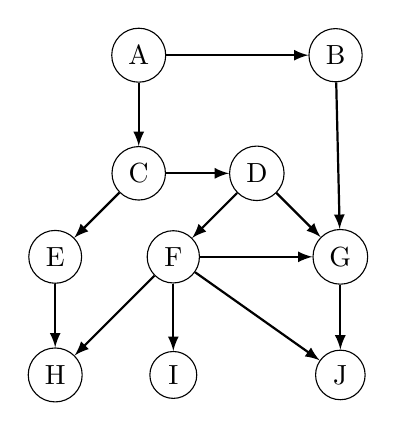
\begin{tikzpicture}
                % cbr = child below right, pbl = parent below left (snippets)
                \tikzset{>=latex}
                \tikzstyle{every node}=[circle, draw=black, node distance=1.5cm]
                \tikzstyle{every edge}=[black, ->, thick, draw]
                \node (A) at (0, 0) {A};
                \node (B) [right of = A, node distance=2.5cm] {B};
                \draw (A) edge (B);
                \node (C) [below of = A] {C};
                \draw (A) edge (C);
                \node (D) [right of = C] {D};
                \draw (C) edge (D);
               \node (E) [below left of = C] {E};
               \draw (C) edge (E);
               \node (H) [below of = E] {H};
               \draw (E) edge (H);
               \node (F) [below left of = D] {F};
               \draw (D) edge (F);
               \node (G) [below right of = D] {G};
               \draw (D) edge (G);
               \draw (F) edge (G);
               \node (I) [below of = F] {I};
               \draw (F) edge (I);
               \node (J) [below of = G] {J};
               \draw (G) edge (J);
               \draw (F) edge (H);
               \draw (F) edge (J);
               \draw (B) edge (G);
        \end{tikzpicture}
        \caption{Complete graph $G$.}
        \label{fig:G2}
\end{figure}

We are interested in the verification of several conditional independence relations. For each 
case, we will verify the relation using Bayes Ball algorithm (see algorithm \ref{alg:Bayes}). 
Here, we exploit the fact that unobserved node do not have the ability to bounce the ball 
when visited by a parent. Therefore, for each cases, we only consider a relevant sub-graph 
of $G$ built by plucking away all the unobserved nodes until an observed node is found or 
a node of interest is found.
\pagebreak
\renewcommand{\arraystretch}{2}
\begin{table}[H]
        \centering
        \begin{tabular}{ccc}
                Relevant sub-graph &  Conditional independence & True/False \\
                \hline
                \begin{tikzpicture}[baseline=(current bounding box.center)]
                        % cbr = child below right, pbl = parent below left (snippets)
                        \tikzstyle{every node}=[circle, draw=black, node distance=1.5cm]
                        \tikzstyle{every edge}=[black, ->, thick, draw]
                        \node (C) at (0, 0) {C};
                        \node (A) [right of = C] {A};
                        \draw (A) edge (C);
                        \node (B) [right of = A] {B};
                        \node[circle, fill=black, inn\
                        \draw (A) edge (B);
                        \draw[<-, blue, dashed, thick, bend right] (C.south east) to 
                                (A.south west);
                        \draw [->, blue, dashed, thick, bend right] (A.south east) to 
                                (B.south west);

                        \draw[->, red, dashed, thick, bend left] (C.north east) to 
                                (A.north west);


                        \draw[->, red, dashed, thick, bend right] (B.north west) to  
                                (A.north east);

                \end{tikzpicture}
                                  & $C \indep B \mid \emptyset$ & False \\
                \cmidrule{2-3}

                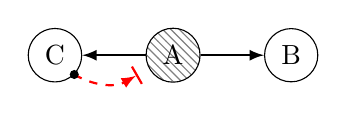
\begin{tikzpicture}[baseline=(current bounding box.center)]

                        % cbr = child below right, pbl = parent below left (snippets)
                        \tikzset{>=latex}
                        \tikzstyle{every node}=[circle, draw=black, node distance=1.5cm]
                        \tikzstyle{every edge}=[black, ->, thick, draw]
                        \node[pattern=north west lines, pattern color=gray] (A) at (0, 0) {A};
                        \node (C) [left of = A] {C};
                        \draw (A) edge (C);
                        \node (B) [right of = A] {B};
                        \draw (A) edge (B);
                        
                        \draw[->|, red, dashed, thick, bend right] (C.south east) to 
                                ([xshift=-0.2cm]A.south west);
                        \node[circle, fill=black, inner sep=1pt] at (C.south east) {};
     %                   \draw [->|, red, dashed, thick, bend left] (B.south west) to 
                                %([xshift=0.2cm]A.south east);
                \end{tikzpicture}
                                  & $C \indep B \mid A $ & True \\
                                  \cmidrule{2-3}
                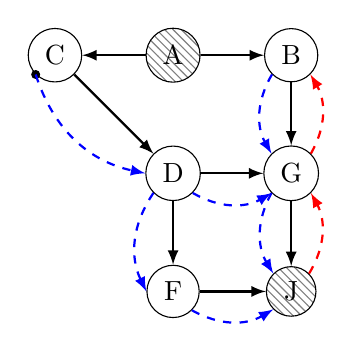
\begin{tikzpicture}[baseline=(current bounding box.center)]
                        % cbr = child below right, pbl = parent below left (snippets)
                        \tikzstyle{every node}=[circle, draw=black, node distance=1.5cm]
                        \tikzstyle{every edge}=[black, ->, thick, draw]
                        \node[pattern=north west lines, pattern color=gray] (A) at (0, 0) {A};
                        
                        \node (C) [left of = A] {C};
                        \node[circle, fill=black, inner sep=1pt] at (C.south west) {};
                        \draw (A) edge (C);
                        \node (B) [right of = A] {B};
                        \draw (A) edge (B);

                        \node (D) [below of = A] {D};
                        \draw (C) edge (D);
                        \node (G) [below of = B] {G};
                        \draw (B) edge (G);
                        \draw (D) edge (G);
                        \node (F) [below of = D] {F};
                        \draw (D) edge (F);
                        \node[pattern=north west lines, pattern color=gray] (J) [below of = G] {J};
                        \draw (G) edge (J);
                        \draw (F) edge (J);

                        
                        \draw [->, blue, dashed, thick, bend right] (C.south west) to 
                                (D.west);

                        \draw[->, blue, dashed, thick, bend right] (D.south west) to 
                                (F.west);

                        \draw[->, blue, dashed, thick, bend right] (D.south east) to 
                                (G.south west);

                        \draw[->, blue, dashed, thick, bend right] (F.south east) to 
                                (J.south west);

                        \draw[->, red, dashed, thick, bend right] (J.north east) to 
                                (G.south east);

                        \draw[->, blue, dashed, thick, bend right] (G.south west) to 
                                (J.north west);

                        \draw[->, red, dashed, thick, bend right] (G.north east) to 
                                (B.south east);


                        \draw[->, blue, dashed, thick, bend right] (B.south west) to 
                                (G.north west);
                        
                        
                \end{tikzpicture}
                                  & $C \indep B \mid A ,J$ & False \\ 
                                  \cmidrule{2-3}

                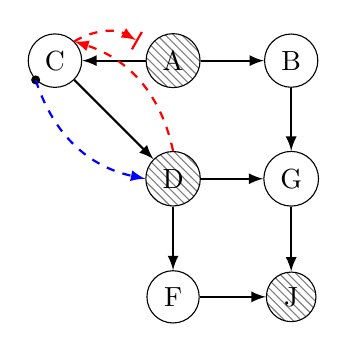
\begin{tikzpicture}[baseline=(current bounding box.center)]
                        % cbr = child below right, pbl = parent below left (snippets)
                        \tikzstyle{every node}=[circle, draw=black, node distance=1.5cm]
                        \tikzstyle{every edge}=[black, ->, thick, draw]
                        \node[pattern=north west lines, pattern color=gray] (A) at (0, 0) {A};
                          
                        \node (C) [left of = A] {C};
                        \draw (A) edge (C);
                        \node (B) [right of = A] {B};
                        \draw (A) edge (B);
                        
                        %\draw[->|, blue, dashed, thick, bend right] (C.south east) to 
                                %([xshift=-0.2cm]A.south west);
                        %\draw [->|, blue, dashed, thick, bend left] (B.south west) to 
                                %([xshift=0.2cm]A.south east);

                        \node[pattern=north west lines, pattern color=gray] (D) [below of = A] {D};
                        \draw (C) edge (D);
                        \node (G) [below of = B] {G};
                        \draw (B) edge (G);
                        \draw (D) edge (G);
                        \node (F) [below of = D] {F};
                        \draw (D) edge (F);
                        \node[pattern=north west lines, pattern color=gray] (J) [below of = G] {J};
                        \draw (G) edge (J);
                        \draw (F) edge (J);
                        \node[circle, fill=black, inner sep=1pt] at (C.south west) {};
                        
                        \draw [->, blue, dashed, thick, bend right] (C.south west) to 
                                (D.west);

                        \draw[->, red, dashed, thick, bend right] (D.north) to 
                                (C.north east);

                        \draw[->|, red, dashed, thick, bend left] (C.north east) to 
                                ([xshift=-0.2cm]A.north west);

                \end{tikzpicture}
                                  & $C \indep B \mid A,J,D$ & True \\
                                  \cmidrule{2-3}
                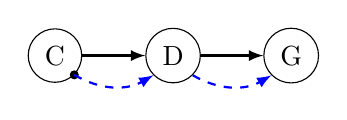
\begin{tikzpicture}[baseline=(current bounding box.center)]
                        % cbr = child below right, pbl = parent below left (snippets)
                        \tikzstyle{every node}=[circle, draw=black, node distance=1.5cm]
                        \tikzstyle{every edge}=[black, ->, thick, draw]
                        \node (C) at (0, 0) {C};
                        \node (D) [right of = C] {D};
                        \draw (C) edge (D);
                        \node (G) [right of = D] {G};
                        \draw (D) edge (G);
                        \node[circle, fill=black, inner sep=1pt] at (C.south east) {};

                        \draw[->, blue, dashed, thick, bend right] (C.south east) to 
                                (D.south west);

                        \draw[->, blue, dashed, thick, bend right] (D.south east) to 
                                (G.south west);

                        %\draw[->, red, dashed, bend right] (G.north west) to 
                                %(D.north east);

                        %\draw[->, red, dashed, bend right] (D.north west) to 
                                %(C.north east);
                        
                \end{tikzpicture}
                                  & C \indep G \mid \emptyset & False \\
                                  \cmidrule{2-3}
                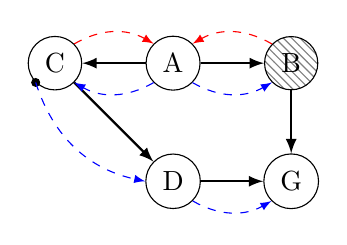
\begin{tikzpicture}[baseline=(current bounding box.center)]
                        % cbr = child below right, pbl = parent below left (snippets)
                        \tikzstyle{every node}=[circle, draw=black, node distance=1.5cm]
                        \tikzstyle{every edge}=[black, ->, thick, draw]
                        \node (A) at (0, 0) {A};
                        \node (C) [left of = A] {C};
                        \node[circle, fill=black, inner sep=1pt] at (C.south west) {};
                        \draw (A) edge (C);
                        \node[pattern=north west lines, pattern color=gray] (B) [right of = A] {B};
                        \draw (A) edge (B);
                        \node (D) [below of = A] {D};
                        \draw (C) edge (D);
                        \node (G) [below of = B] {G};
                        \draw (B) edge (G);
                        \draw (D) edge (G);

                        \draw[->, blue, dashed, bend right] (C.south west) to 
                                (D.west);

                        \draw[->, blue, dashed, bend right] (D.south east) to 
                                (G.south west);

                        \draw[->, red, dashed, bend left] (C.north east) to 
                                (A.north west);

                        \draw[->, blue, dashed, bend right] (A.south east) to 
                                (B.south west);

                        \draw[->, red, dashed, bend right] (B.north west) to 
                                (A.north east);


                        \draw[->, blue, dashed, bend left] (A.south west) to 
                                (C.south east);
                \end{tikzpicture}
                                  & $C \indep G \mid B$ & False \\
                          \cmidrule{2-3}
                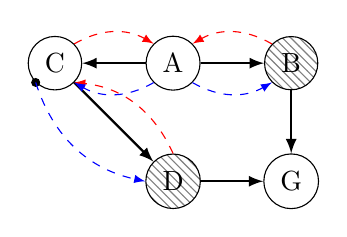
\begin{tikzpicture}[baseline=(current bounding box.center)]
                        % cbr = child below right, pbl = parent below left (snippets)
                        \tikzset{>=latex}
                        \tikzstyle{every node}=[circle, draw=black, node distance=1.5cm]
                        \tikzstyle{every edge}=[black, ->, thick, draw]
                         \node (A) at (0, 0) {A};
                        \node (C) [left of = A] {C};
                        \node[circle, fill=black, inner sep=1pt] at (C.south west) {};
                        \draw (A) edge (C);
                        \node[pattern=north west lines, pattern color=gray] (B) [right of = A] {B};
                        \draw (A) edge (B);
                        \node[pattern=north west lines, pattern color=gray] (D) [below of = A] {D};
                        \draw (C) edge (D);
                        \node (G) [below of = B] {G};
                        \draw (B) edge (G);
                        \draw (D) edge (G);

                        \draw[->, blue, dashed, bend right] (C.south west) to 
                                (D.west);

                        \draw[->, red, dashed, bend right] (D.north) to 
                                (C.south east);


                        \draw[->, red, dashed, bend left] (C.north east) to 
                                (A.north west);

                        \draw[->, blue, dashed, bend right] (A.south east) to 
                                (B.south west);

                        \draw[->, red, dashed, bend right] (B.north west) to 
                                (A.north east);


                        \draw[->, blue, dashed, bend left] (A.south west) to 
                                (C.south east);
                        
                \end{tikzpicture}
                                  & $C \indep G \mid B, D$ & True\\
                                  \cmidrule{2-3}
                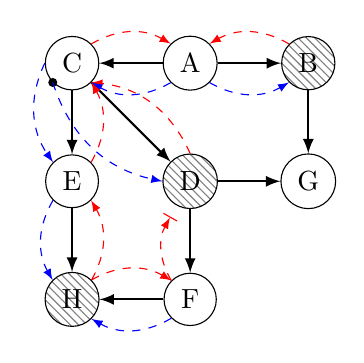
\begin{tikzpicture}[baseline=(current bounding box.center)]
                        % cbr = child below right, pbl = parent below left (snippets)
                        \tikzset{>=latex}
                        \tikzstyle{every node}=[circle, draw=black, node distance=1.5cm]
                        \tikzstyle{every edge}=[black, ->, thick, draw]
                        \node (A) at (0, 0) {A};
                        \node (C) [left of = A] {C};
                        \node[circle, fill=black, inner sep=1pt] at (C.south west) {};
                        \draw (A) edge (C);
                        \node[pattern=north west lines, pattern color=gray] (B) [right of = A] {B};
                        \draw (A) edge (B);
                        \node[pattern=north west lines, pattern color=gray] (D) [below of = A] {D};
                        \draw (C) edge (D);
                        \node (G) [below of = B] {G};
                        \draw (B) edge (G);
                        \draw (D) edge (G);
                        \node (E) [below of = C] {E};
                        \draw (C) edge (E);
                        \node[pattern=north west lines, pattern color=gray] (H) [below of = E] {H};
                        \draw (E) edge (H);
                        \node (F) [below of = D] {F};
                        \draw (D) edge (F);
                        \draw (F) edge (H);
                        
                      \draw[->, blue, dashed, bend right] (C.south west) to 
                                (D.west);

                        \draw[->, red, dashed, bend right] (D.north) to 
                                (C.south east);


                        \draw[->, red, dashed, bend left] (C.north east) to 
                                (A.north west);

                        \draw[->, blue, dashed, bend right] (A.south east) to 
                                (B.south west);

                        \draw[->, red, dashed, bend right] (B.north west) to 
                                (A.north east);


                        \draw[->, blue, dashed, bend left] (A.south west) to 
                                (C.south east);

                        \draw[->, blue, dashed, bend right] (C.west) to 
                                (E.north west);

                        \draw[->, blue, dashed, bend right] (E.south west) to 
                                (H.north west);

                        \draw[->, red, dashed, bend right] (H.north east) to 
                                (E.south east);

                        \draw[->, red, dashed, bend right] (E.north east) to 
                                (C.south east);

                        \draw[->, red, dashed, bend left] (H.north east) to 
                                (F.north west);
                        
                        \draw[->|, red, dashed, bend left] (F.north west) to 
                                ([yshift=-0.2cm]D.south west);

                        \draw[->, blue, dashed, bend left] (F.south west) to 
                                (H.south east);
                        
                \end{tikzpicture}
                                  & $C \indep G \mid B, D, H$ & True \\
                                  \cmidrule{2-3}

                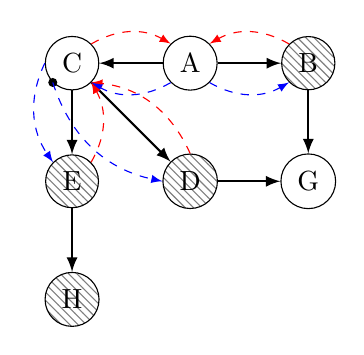
\begin{tikzpicture}[baseline=(current bounding box.center)]
                        % cbr = child below right, pbl = parent below left (snippets)
                        \tikzset{>=latex}
                        \tikzstyle{every node}=[circle, draw=black, node distance=1.5cm]
                        \tikzstyle{every edge}=[black, ->, thick, draw]
                        \node (A) at (0, 0) {A};
                        \node (C) [left of = A] {C};
                        \node[circle, fill=black, inner sep=1pt] at (C.south west) {};
                        \draw (A) edge (C);
                        \node[pattern=north west lines, pattern color=gray] (B) [right of = A] {B};
                        \draw (A) edge (B);
                        \node[pattern=north west lines, pattern color=gray] (D) [below of = A] {D};
                        \draw (C) edge (D);
                        \node (G) [below of = B] {G};
                        \draw (B) edge (G);
                        \draw (D) edge (G);
                        \node[pattern=north west lines, pattern color=gray] (E) [below of = C] {E};
                        \draw (C) edge (E);
                        \node[pattern=north west lines, pattern color=gray] (H) [below of = E] {H};
                        \draw (E) edge (H);
                      \draw[->, blue, dashed, bend right] (C.south west) to 
                                (D.west);

                        \draw[->, red, dashed, bend right] (D.north) to 
                                (C.south east);


                        \draw[->, red, dashed, bend left] (C.north east) to 
                                (A.north west);

                        \draw[->, blue, dashed, bend right] (A.south east) to 
                                (B.south west);

                        \draw[->, red, dashed, bend right] (B.north west) to 
                                (A.north east);


                        \draw[->, blue, dashed, bend left] (A.south west) to 
                                (C.south east);

                        \draw[->, blue, dashed, bend right] (C.west) to 
                                (E.north west);


                        \draw[->, red, dashed, bend right] (E.north east) to 
                                (C.south east);

                                               
                \end{tikzpicture}
                                  & $C \indep G \mid B, D, H, E$ & True \\
                                  \hline
                
                
                
        \end{tabular}
        \caption{Conditional independence statements and active trail 
        (blue dashed paths) shown in the relevant path column for questions (a) to 
        (i).}
        \label{tab:CondIndep1}
\end{table}
\pagebreak 

\begin{table}[H]
        \centering
        \begin{tabular}{ccc}
                Relevant sub-graph &  Conditional independence & True/False \\
                \hline
                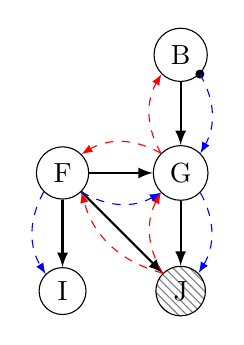
\begin{tikzpicture}[baseline=(current bounding box.center)]
                        % cbr = child below right, pbl = parent below left (snippets)
                        \tikzset{>=latex}
                        \tikzstyle{every node}=[circle, draw=black, node distance=1.5cm]
                        \tikzstyle{every edge}=[black, ->, thick, draw]
                        \node (B) at (0, 0) {B};
                        \node (G) [below of = B] {G};
                        \draw (B) edge (G);
                        \node[pattern=north west lines, pattern color=gray] (J) [below of = G] {J};
                        \draw (G) edge (J);
                        \node (F) [left of = G] {F};
                        \draw (F) edge (G);
                        \node (I) [below of = F] {I};
                        \draw (F) edge (I);
                        \draw (F) edge (J);
                        \node[circle, fill=black, inner sep=1pt] at (B.south east) {};


                        \draw[->, blue, dashed, bend left] (B.south east) to 
                                (G.north east);
                        
                        \draw[->, blue, dashed, bend left] (G.south east) to 
                                (J.north east);

                        \draw[->, red, dashed, bend left] (J.north west) to 
                                (G.south west);

                        \draw[->, red, dashed, bend left] (J.north west) to 
                                (F.south east);


                        \draw[->, red, dashed, bend right] (G.north west) to 
                                (F.north east);


                        \draw[->, red , dashed, bend left] (G.north west) to 
                                (B.south west);

                        
                        \draw[->, blue, dashed, bend right] (F.south west) to 
                                (I.north west);

                        \draw[->, blue, dashed, bend right] (F.south east) to 
                                (G.south west);
                \end{tikzpicture}
                                   & $B \indep I \mid J$ & False \\
                                   \hline
                
        \end{tabular}
        \caption{Conditional independence statement of question (j). In the relevant 
        sub-graph we omitted the node $D$ because we wanted to show the shortest active 
                trail.}
        \label{tab:CondIndep2}
\end{table}

\section{Appendix}
\subsection{Bayes Ball algorithm}
Here we focus our attention to the Bayes Ball algorithm for probabilistic node only. In that 
case, conditional independence $X_J \indep X_L \mid X_K$, with $J,K,L \subseteq V$ requires 
the notion of d-separation:
\begin{description}
        \item{\textbf{Active path}} An active path from $J$ to $L$ given $K$ is 
                an undirected path between $\ell \in L$ and $j \in J$ such that every 
                node $i$ with two parents in this chain is observed ($i \in K$) or 
                has a descendant in $K$ ($i \in K \cap \text{descendant}(i)$)
        \item{\textbf{D-separation}} $X_j$ is said to be conditionally independent to 
                $X_L$ (or 
                \textit{d-separate} $X_L$) given $X_K$ if there is no active path 
                from $J$ to $L$ given $K$.
\end{description}
With this description, we can devise a simple algorithm that will find all active 
path in the graph in linear time \cite{BB}. We will use the following convention 
\begin{itemize}
        \item $\color{blue} \dashrightarrow $ Dashed blue arrows indicate the ball drop from parent to child;
        \item $\color{red} \dashrightarrow$ Dashed red arrow indicate the ball bounce back to the 
                parent;
        \item Barred arrows mean the node will block the ball (neither bounce it back 
                nor let it pass through). These can be used as an indicator and are not 
                necessary for the algorithm.
\end{itemize}
With this convention, we describe an algorithm that will find all active path 
from a node $\ell \in L$ to a node $j \in J$ given 
$K$ if they exists:

\begin{algorithm}[H]
        \KwResult{active paths in the graph $\color{blue} \dashrightarrow$}
        initialize a schedule with all $j \in J$ as though they were  
        visited by a child\;
        \While{schedule not empty}{ 
                pick a node $j$ and remove it from the schedule\;
                \If{$j \not\in K$ \textbf{and} 
                        $j$ is visited from a child \textbf{and} there is no 
                        $\color{red} \dashrightarrow$ linking $j$ to previous node}{
                        draw $\color{red} \dashrightarrow$ going into $j$\;
                        schedule its parents to be visited\;
                        schedule its children to be visited\;
                }
                \uElseIf{$j$ is visited from a parent \textbf{and} there is no 
                        $\color{blue} \dashrightarrow$ linking $j$ to previous node}{
                        draw $\color{blue} \dasharrow$ going into $j$\;
                        \eIf{$j \in K$}{
                                schedule its parents to be visited\;
                        }{
                        schedule its children to be visited\;
                }
                        
        }
        }

        \caption{Bayes Ball} 
        \label{alg:Bayes}
\end{algorithm}
%With this description of conditional independence, a simple algorithm given only 
%two simple rules:
%\begin{itemize}
        %\item An unobserved node pass the ball through and bounce it back to its 
                %parent;
        %\item An observed node bounce back the ball from the parents, and block the 
                %ball for the children.
%\end{itemize}
%To determine we start from a node in $J$ and search for an active path that leads to $L$ 
%given $K$.



\begin{thebibliography}{9}
        \bibitem{BB}
        Shachter, R. D. (2013). 
        Bayes-Ball: The Rational Pastime (for Determining Irrelevance and Requisite Information in Belief Networks and Influence Diagrams). \url{http://arxiv.org/abs/1301.7412}
        
\end{thebibliography}

\end{document}

